\section{Theorie}
\label{sec:Theorie}
%Bei einer Besetzungsinversion wird die induzierte Abkehr von der thermischen Besetzungswahrscheinlichkeit der Energieniveaus eines Atoms herbeigeführt.
%Um dies zu verstehen ist es zunächst nötig, die elektronische Struktur des hier untersuchten Elements Rubidium zu erläutern.

\subsection{Beschreibung der Energieniveaus in Rubidium}
\label{subsec:energieniveaus}

Bei Rubidium handelt es sich um ein Alkalimetall, das nur über ein ungepaartes Elektron in der fünften Schale verfügt, sodass nur dieses zu den Quantenzahlen der Elektronenhülle beiträgt.
Ohne Betrachtung von Korrekturen befindet es sich als Spin-1/2-Teilchen in dem Zustand mit $n=5$, $L=0$ und $M_L=0$. Dabei ist $n$ die Hauptquantenzahl, $L$ die Drehimpulsquantenzahl und $M_L$ die zu ihr gehörige magnetische Quantenzahl. \\
Die Zustände sind entartet. Diese Entartung kann durch die Feinstruktur, die Hyperfeinstruktur und den Zeeman-Effekt aufgehoben werden (vergleiche Abbildung \ref{fig:energieniveaus}).
%In niedrigster Ordnung verfügt das Niveau mit $L=1$ und $M_L=0,\pm1$ über die gleiche Energie wie der besetzte Zustand. Sie sind entartet.\\

\begin{figure}
  	\centering
  	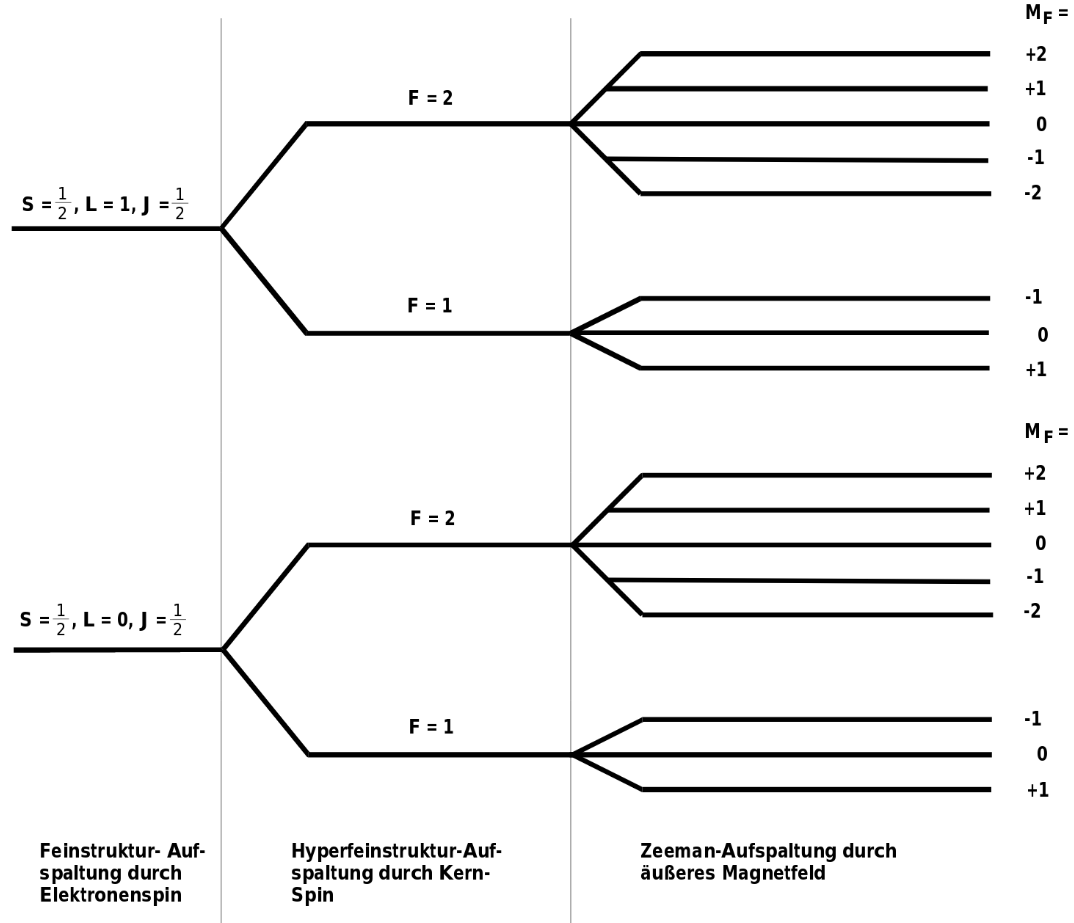
\includegraphics[width=0.88\textwidth,keepaspectratio]{content/images/energieniveaus.png}
  	\caption{Energieniveaus in \ce{^{87}Rb} mit $I=3/2$ (nicht maßstäblich) \cite{alt}.}
  	\label{fig:energieniveaus}
\end{figure}

\subsubsection{Elektronenspin und Feinstruktur}
Der Gesamtdrehimpuls $\vec{J}$ einer Elektronenhülle eines Atoms setzt sich aus Bahndrehimpuls $\vec{L}$ und Spin $\vec{S}$ wie folgt zusammen:
\begin{equation*}
  \vec{J} = \vec{L} + \vec{S} \text{.}
\end{equation*}
Dies kommt durch die Spin-Bahn-Kopplung des Elektronenspins zustande.
Die Quantenzahlen $J$ und $M_J$ definieren nun statt $L$ und $M_L$ einen gegebenen Zustand, wobei $J$ von $\lvert L - S \rvert$ bis $\lvert L + S \rvert$ reicht. Zustände mit verschiedenem $J$ sind in dieser Feinstruktur nicht mehr energetisch entartet, während Zustände mit gleichem $J$ und verschiedenem $M_J$ ohne äußeres Magnetfeld energetisch entartet bleiben.

\subsubsection{Kernspin und Hyperfeinstruktur}
Die Niveaus werden in eine weitere Hyperfeinstruktur aufgespalten, wenn die Spin-Spin-Kopplung des Kernspins an den Gesamtdrehimpuls der Elektronenhüllen berücksichtigt wird. Es ergibt sich für den Gesamtdrehimpuls $\vec{F}$ des Atoms:
\begin{equation*}
  \vec{F} = \vec{J} + \vec{I} \text{.}
\end{equation*}
Zu diesem gehört die Quantenzahl $F$, die Werte von $\lvert J - I \rvert$ bis $\lvert J + I \rvert$ annimmt, mit der magnetischen Quantenzahl $M_F$. 
%In Abbildung \ref{fig:energieniveaus} werden die Feinstrukturniveaus dementsprechend jeweils in zwei Niveaus aufgespalten, wobei wieder Zustände mit gleichem $F$ und verschiedenem $M_F$ ohne äußeres Magnetfeld energetisch entartet bleiben.\\

\subsubsection{Der Zeeman-Effekt}
Die Aufhebung der Entartung dieser Zustände durch ein Magnetfeld geschieht durch den sogenannten Zeeman-Effekt. Dieser spaltet einen $F$-Zustand wiederum in $2F$+1-Zustände auf. Die Energiedifferenz zweier benachbarter Zeeman-Niveaus beträgt
\begin{equation}
\Delta E_Z = g_F \mu_{\text{B}} B
\label{eqn:zeemanDifferenz}
\end{equation}
und ist somit proportional zur magnetischen Flussdichte $B$. Der Faktor $\mu_{\text{B}} = \frac{e \hbar}{2m_e}$ ist das Bohrsche Magneton.\\
Der Landé-Faktor des Gesamtdrehimpulses des Atoms $g_F$ ergibt sich aus Kopplungsdiagrammen der beteiligten Drehimpulse näherungsweise zu
\begin{equation}
g_F = g_J \frac{F(F+1)+J(J+1)-I(I+1)}{2F(F+1)}\,,
\label{eqn:g_F_Theorie}
\end{equation}
wobei der Landé-Faktor des Gesamtdrehimpulses des Elektrons $g_J$ gegeben ist durch:
\begin{equation}
g_J = \frac{3{,}0023J(J+1)+1{,}0023(S(S+1)-L(L+1))}{2J(J+1)}
\label{eqn:g_J_Theorie}
\end{equation}

\subsubsection{Abschätzung des quadratischen Zeeman-Effekts}
\label{subsec:quadratischerZeeman}

%Um Felder mittlerer Stärke zu betrachten, werden weitere Ordnungen der Störungstheorie bei der Berechnung des Zeeman-Effekts berücksichtigt. In niedrigster Ordnung ist dies dann der quadratische Zeeman-Effekt, sodass die Energiedifferenz aus Gleichung \eqref{eqn:zeemanDifferenz} zu
Im Falle großer Magnetfelder entstehen aufgrund der Wechselwirkungen des Spins mit dem Bahndrehimpuls und der Wechselwirkung der magnetischen Momente weitere Effekte, welche bei der Zeemann-Aufspaltung berücksichtigt werden müssen. In niedrigster Ordnung Störungstheorie ist dies dann der quadratische Zeeman-Effekt.
Es ergibt sich für die Zeemann-Aufspaltung als Erweiterung von Formel \eqref{eqn:zeemanDifferenz}:
\begin{equation}
\Delta E_Z = g_F \, \mu_{\text{B}} B + g_F^2 \, \mu_{\text{B}}^2 B^2 \frac{1-2M_F}{\Delta E_{\text{Hy}}},
\label{eqn:zeemanDifferenzQuadratisch}
\end{equation}
wobei $E_\text{Hy}$ die Hyperfeinstrukturaufspaltung zwischen den Niveaus zwischen $F$ und $F+1$ bezeichnet.


\subsection{Optisches Pumpen}
\label{subsec:prinzipOptischesPumpen} 

\subsubsection{Prinzip des optischen Pumpens}

%Es ist üblich, die Feinstrukturniveaus als Termsymbole ${}^{2S+1}L_J$ mit der Multiplizität $2S+1$ und dem Kennbuchstaben $L$ für den elektronischen Drehimpuls zu schreiben, wobei für $L=0$ ein S und für $L=1$ ein P geschrieben wird.
Beim optischen Pumpen werden die Niveaus entegegen der thermischen Verteilung besetzt.
%Es ist also möglich, die Verteilung der äußeren Hüllenelektronen zu invertieren.
Für das optische Pumpen an Rubidium ist die Aufspaltung der Hyperfeinstrukturniveaus durch den Zeeman-Effekt nötig. Die Besetzung folgt dann näherungsweise einer thermischen Boltzmann-Verteilung, sodass die Elektronen größtenteils im Grundzustand mit niedrigstem $m_F$ angereichert sind.\\
In diesem Versuch wird rechtszirkular polarisiertes Licht der Frequenz des $D_1$-Übergangs eingestrahlt. Übergänge, die durch Absorption dieser Photonen entstehen (stimulierte Emission) gehorchen der Auswahlregel $\Delta M_F=+1$, während die spontane Emission keine bestimmten Übergänge bevorzugt. Dadurch werden die unteren Niveaus entleert und der S-Zustand mit $F=2$, $M_F=2$ angereichert. Es wird eine Besetzungsinversion herbeigeführt. Eine schematische Darstellung der Übergänge findet sich in Abbildung \ref{fig:pumpschema}.

\begin{figure}
	\centering
	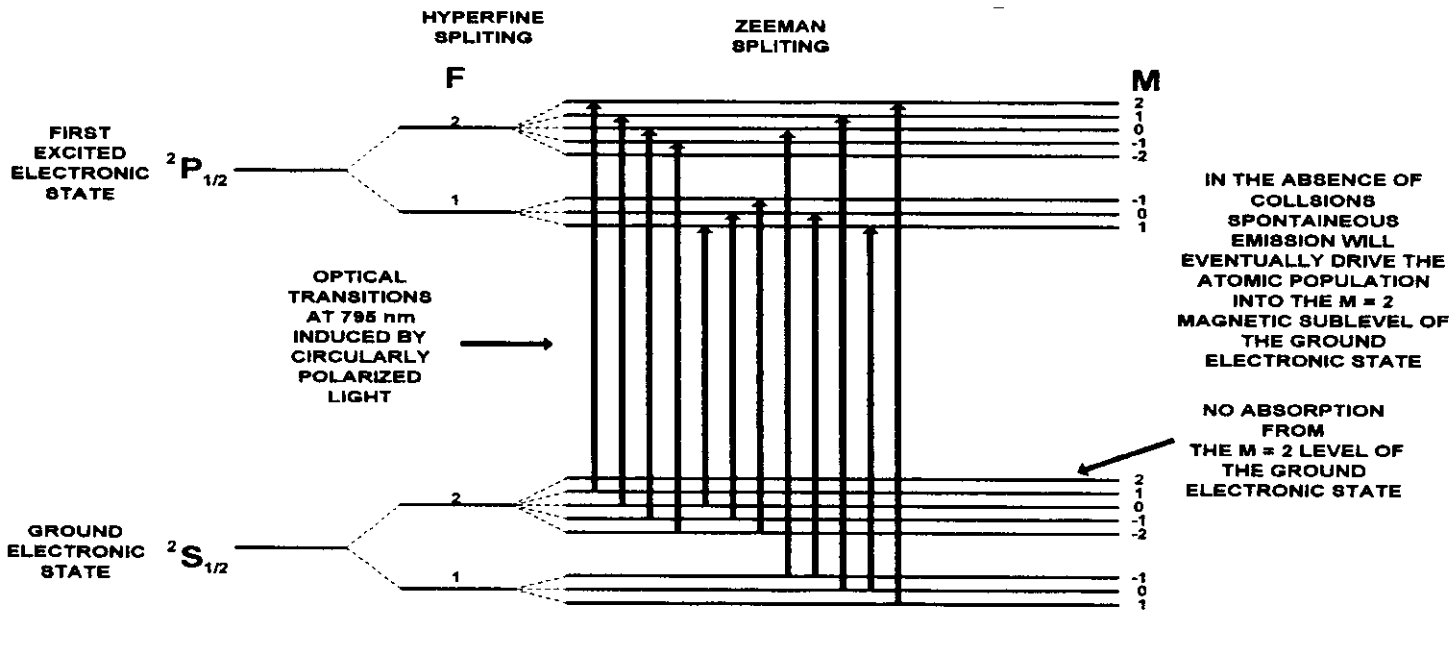
\includegraphics[width=0.96\textwidth,keepaspectratio]{content/images/pumpschema.png}
	\caption{Pumpschema für \ce{^{87}Rb} ($I=3/2$) zur Herstellung einer Besetzungsinversion \cite{caltech}.}
    \label{fig:pumpschema}
\end{figure}

\noindent Ein geeignetes Maß für die Besetzungsinversion stellt die Transparenz der Dampfzelle gegenüber dem einstrahlenden $D_1$-Licht dar. Diese wird mit einer ansteigenden Exponentialfunktion parametrisiert, welche sich bei vollständiger Inversion sättigt.\\

\subsubsection{Einfluss eines hochfrequenten magnetischen Feldes}
Optischen Pumpen wird oft als spektroskopisches Verfahren eingesetzt, um die aufgespaltenen Energieniveaus mit hoher Genauigkeit zu vermessen. Dieses Messverfahren bedient sich eines zweiten, hochfrequenten magnetischen Feldes (RF-Feld), welches stimulierte Emission aus dem angereicherten Niveau heraus anregt. Für die dafür benötigte Flussdichte $B_m$ gilt die Beziehung
\begin{equation}
h f = g_F \, \mu_{\text{B}} B_m \Delta M_F \implies B_m = \frac{4 \pi m_e}{e g_F} f
\label{eqn:B_M_Theorie}
\end{equation}
%sodass ein linearer Zusammenhang zu der Frequenz des Feldes besteht.
Da mit der stimulierten Emission eine Entleerung des zuvor angereicherten Niveaus verbunden wird, ist das Erreichen der Feldstärke $B_m$ mit einer deutlichen Abnahme der Transparenz des Gases verbunden. %, weil der konkurrierende Prozess der Besetzungsinversion durch optisches Pumpen wieder aufnehmen kann (vergleiche Abbildung \ref{fig:transparenz}).\\
Um 0 herum sinkt die Transparenz ebenfalls deutlich ab, da es ohne Äußeres Magnetfeld nicht zu einer Zeeman-Aufspaltung kommen kann (vergleiche Abbildung \ref{fig:transparenz}). %Experimentell wird dies ausgenutzt, um den Einfluss des Erdmagnetfelds zu minimieren.

\begin{figure}
    \centering
    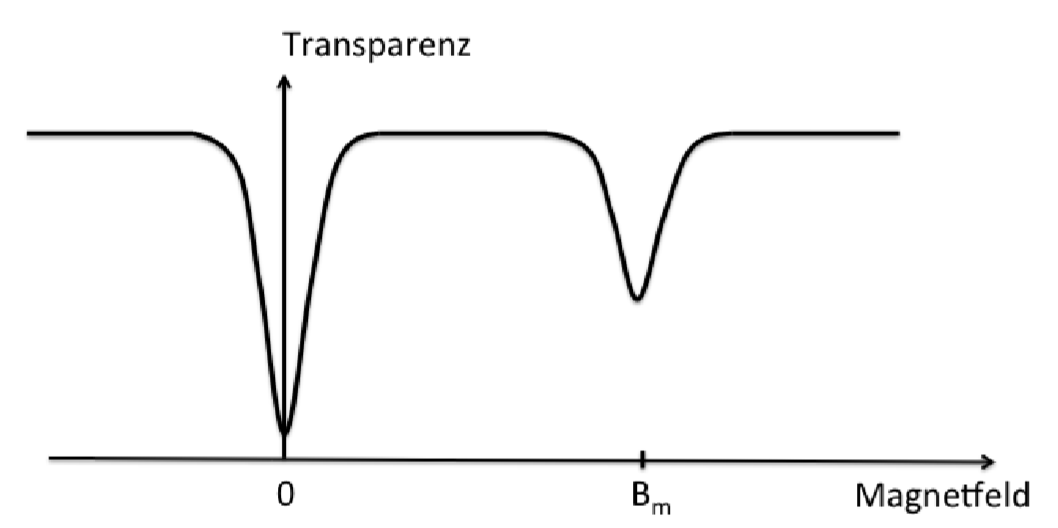
\includegraphics[width=\textwidth-120pt,keepaspectratio]{content/images/transparenz.png}
  	\caption{Transparenz der Dampfzelle in Abhängigkeit eines äußeren Magnetfelds \cite{V21}.}
    \label{fig:transparenz}
\end{figure}

\newpage
\subsubsection{Transiente Effekte}
\label{subsec:transient}

Beim schnellen Ein- und Ausschalten des RF-Feldes zeigt sich, dass der Spin $\vec{F}$ im rotierenden Koordinatensystem um die Achse des RF-Feldes präzediert, wenn das statische Magnetfeld resonant eingestellt ist. Die Lamor-Frequenz beträgt dabei $\gamma B_{\text{RF}}$ mit dem gyromagnetischen Verhältnis 
\[
\gamma = g_F \frac{\mu_{\text{B}}}{\hbar},
\]
sodass die Periodendauer der sogenannten Rabi-Oszillation 
\[
T=\frac{1}{(\gamma B_\text{RF})}
\]
amplitudenabhängig ist.
Es gilt:
\begin{equation}
\frac{T_{87}}{T_{85}} = \frac{\gamma_{85}}{\gamma_{87}}
\label{eqn:transient}
\end{equation}

\subsection{Helmholtzspule}

Helmholtzspulen erzeugen in ihrem inneren ein nahezu homogenes Magnetfeld $B$. Dieses wird berechnet über:
\begin{equation}
B = \mu_0\frac{8}{\sqrt{125}}\frac{IN}{R},
\label{eq:helmholtz}
\end{equation}
mit der magnetischen Feldkonstanten $mu_0$, der Windungszahl $N$ und dem Radius $R$ der Spule, sowie dem angelegten Strom $I$.